In questo capitolo verranno trattate le metodologie con cui si è deciso di approfondire con l'analisi del tx-graph. In particolare si è preferito adottare un approccio più incentrato sullo studio degli andamenti e della frequenza delle varie catene di transazioni.

\section{Networkx per la creazione di grafi}

Per questo progetto, si è deciso di utilizzare il linguaggio di programmazione Python, in aggiunta con l'utilizzo di varie librerie, in particolare \textit{Networkx}, la quale permette la creazione, la gestione e l'analisi dei grafi. 

Alcune caratteristiche di tale libreria sono:
\begin{itemize}
	\item Strutture dati per grafi diretti, indiretti
	\item Molti algoritmi standard per la gestione dei grafi
	\item Software open soruce
\end{itemize}

Per la gestione di un grafo come il tx-graph, ovvero un grafo generato da tutte le transazioni dei blocchi che vengono considerati nel dataset, si è deciso di utilizzare un \textit{MultiDiGraph}, un grafo diretto con auto archi ed archi paralleli.

\section{Dataset}

Il dataset utilizzato è un insieme di blocchi reali. Essi sono stati scaricati precedentemente e salvati su file in formato json. Ogni singolo blocco è caratterizzato da un numero, il numero che caratterizza l'ordine nella blockchain, e il file che rappresenta i dati di tale blocco ha il nome che corrisponde a tale numero con l'estensione \textit{.json}.

\subsection{Struttura dati di un blocco}
Per ogni blocco, esiste un file \textit{<numblocco>.json}, con determinate caratteristiche. 

\begin{lstlisting}[basicstyle=\tiny, caption = \textit{Prime righe del file 417113.json}, label=417113]
{"txs": [{
	"valueOut": 25.29311068,
	"isCoinBase": true,
	"vout": [{ ... }],	
	"blockhash": "000000000000000002fa1d0daee52356ca68a5964efc389e237a5cf589fe82d6",
	"vin": [{ ... }],
	"txid": "c4be4eda4bb0fce550f89b7ed00d1202a8dd41bb62c2a1254b61b96b0c3e627b",
	"blocktime": 1466381104,
	"version": 1,
	"confirmations": 59748,
	"time": 1466381104,
	"blockheight": 417113,
	"locktime": 863856133,
	"size": 185
},
{
	"valueOut": 2.39,	
	"vout": [{ ... }],	
	"blockhash": "000000000000000002fa1d0daee52356ca68a5964efc389e237a5cf589fe82d6",
	"valueIn": 2.4,
	"fees": 0.01,	
	"vin": [{ ... },{ ... }],
	"txid": "d064980449192201f5d23cf8f6a4fec1dddff58ec9d6692c8996c1007b98250a",	
	"blocktime": 1466381104,
	"version": 1,
	"confirmations": 59748,
	"time": 1466381104,
	"blockheight": 417113,
	"locktime": 0,
	"size": 339
},
\end{lstlisting}

Nel codice \ref{417113}, vengono indicate solamente le prime righe del file 417113.json. Dal momento che un file di questo tipo rappresenta un singolo blocco, al suo interno si potrà trovare una lista di transazioni. Il file, essendo ti tipo json, viene rappresentato come un dizionario in cui i dati sono rappresentati nel formato chiave-valore.

Nella riga 1, al corrispondere dell'attributo "txs" si ha una lista di transazioni. Dal momento che queste sono le prime righe del file, la prima transazione di un blocco è essenzialmente quella generata dal miner quando il blocco viene minato. Di conseguenza come prima transazione si troverà sempre un oggetto che avrà il campo "isCoinBase" uguale a True, che sta a significare che tale transazione è la prima del blocco e non ha transazioni in entrata.

Dal secondo oggetto della lista in poi, si ha una configurazione standard per tutte le altre transazioni che fanno parte del blocco. Come primo campo si ha "valueOut", il quale indica il valore totale di bitcoin che vengono emessi dalla transazione. Il campo "vout" rappresenta invece la lista di transazioni verso le quali gli output vengono spesi. Esiste anche il campo "vin" che raccoglie la lista delle transazioni di cui gli output vengono spesi dalla transazione in questione. 

Il campo "txid" rappresenta l'id della transazione, ovvero il principale identificativo dell'oggetto preso in considerazione. 

Nella singola transazione, si possono notare anche parametri che indicano attributi legati all'appartenenza al blocco:
\begin{itemize}
	\item "blockhash" rappresenta l'identificativo hash del blocco di appartenenza della transazione
	\item "blocktime" è il timestamp del blocco
	\item "blockheight" è il numero che identifica il blocco all'interno della blockchain (in questo caso "blockheight" = 417113)
\end{itemize}
Inoltre, si può notare anche il campo "fees" che rappresenta appunto le fee (cioè le tasse), che tale transazione versa al miner che è riuscito a minare la blockchain.

Nell'esempio del codice sopra citato, vengono riscritte le prime righe del file json, che comprendono le prime due transazioni del blocco. In realtà, come si è già sottolineato, la il primo oggetto della lista è la transazione che fornisce la ricompensa al miner, non è una transazione vera e propria. Perciò il codice visualizza solamente la prima transazione vera e propria, che è la seconda nella lista di oggetti.

Per ogni transazione sono conservati anche i parametri del blocco di appartenenza, come il numero del blocco, il suo codice hash e il suo timestamp. Naturalmente tali parametri sono uguali per tutte le transazioni dello stesso blocco. Tutto ciò facilita molto l'analisi e la creazione del tx-graph poichè ogni transazione ha già il parametro del blocco di appartenenza, senza bisogno di creare ulteriori strutture dati.

Questo esempio riguarda solamente una transazione di un blocco, ma l'analisi in questione viene fatta prendendo in considerazione al più 1000 blocchi, che vengono tutti letti come file json.

Si considerino due possibili situazioni: inizialmente è stata fatta un'analisi su un primo dataset che comprende i blocchi dal 417113 al 417256, proprio come nel paper \cite{ddp-ltcbh-17}. Successivamente, come nel suddetto paper, vengono considerati i blocchi dal 413000 al 419143. I due dataset hanno lo scopo di rappresentare intervalli di tempo diversi. Infatti il primo, sta a rappresentare l'attività di emissione di transazioni che comprende 24 ore. Il secondo invece, rappresenta quanto una macchina può computare al livello di memoria. Per motivi di efficienza e mancanza di risorse computazionali elevate, il secondo dataset è stato ridotto a solamente 1000 blocchi, ovvero dal 413000 al 414000. In questo modo, anche con il secondo dataset è stato possibile generare dei risultati adeguati che poi sono stati infine graficati, per osservare meglio gli andamenti e le periodicità più importanti.

Perciò vengono definiti due dataset $D1=(417113,417256)$ e $D2=(413000,414000)$, che successivamente verranno utilizzati per creare i grafi $G1=G(417113,417256)$ e $G2=G(413000,414000)$.

\section{Cammino più lungo a varianza minima}

Come è stato ampiamente illustrato nel capitolo precedente, l'analisi del grafo delle transazioni verte specialmente sul problema di trovare un cammino, ovvero una catena di transazioni, tale che sia il più lungo e contemporaneamente sia a varianza minima.

Si è deciso di considerare questi parametri, proprio perchè è possibile che il risultato restituito sia proprio corrispondente ad una catena di transazioni generate automaticamente da un mixer. Purtroppo questo processo di verifica, non permette di essere certi di quello che si sta valutando, ma potrebbe porre le fondamenta per un successivo studio approfondito di tali comportamenti.

Per calcolare il cammino più lungo a varianza minima è stato definito un algoritmo. Esso effettua un'analisi sul grafo delle transazioni che viene creato nel prossimo paragrafo.

\subsection{Creazione grafo delle transazioni}
Prima di parlare dell'algoritmo, verrà illustrato come sono stati letti i dati e come viene creato il grafo.

Utilizzando le funzioni di networkx, diventa semplice costruire un grafo in python. Infatti basta usufruire delle funzioni di tale libreria.

Il metodo che crea il grafo prende in input i numeri dei blocchi come range, e legge, in ordine, tutti i file json. Leggendo i singoli json, crea una lista di oggetti, dove ogni oggetto è un blocco con la rispettiva lista di transazioni. Dopo la lettura, viene iterato sulla lista di blocchi, viene presa la lista di transazioni, e vengono creati i nodi del grafo, dove ogni nodo corrisponde ad una transazione.

Per creare gli archi, si cicla su tutte le transazioni e si legge il campo "vin" e "vout". Rispettivamente, il primo indica gli archi entranti in quella transazione,e il secondo gli archi uscenti. In base a questi campi, si cicla sulle due liste "vin" e "vout" e si verifica che le transazioni presenti in tali liste siano corrisposte da una loro rappresentazione all'interno del grafo sotto forma di nodi. 

Ovviamente, se si considera un numero limitato di blocchi, è molto probabile, che singole transazioni vengano rappresentate esclusivamente da un singolo nodo che costituisce una componente a sè stante. Infatti è importante gestire le eccezioni in questo caso specifico.

Nel codice seguente, si può osservare la modalità di creazione del grafo.


\begin{lstlisting}[basicstyle=\tiny]
def create_graph(start_block, end_block):
	blocks = read_blocks(start_block, end_block)	
	G = nx.MultiDiGraph()
	ts = blocks[0]['ts'], dic ={}
	for i in blocks:
		for j in i['txs']:
		count = count+1
		temptxid = j['txid']
		G.add_node(count, txid=temptxid, blockhash=i['blockhash'], 
				numblock=i['numblock'],blocktime=i['blocktime'], ts=0)
		dic[temptxid] = count
		currId = dic[j['txid']]
			for k in j['vout']:
				try:
					outNodeId = dic[k['spentTxId']]	
					if not G.has_edge(currId, outNodeId):
						G.add_edge(currId, outNodeId)
				except KeyError: break	
			for h in j['vin']:
				try:
					inNodeId = dic[h['txid']]
					if not G.has_edge(inNodeId, currId):
						G.add_edge(inNodeId, currId)
				except KeyError: break	
\end{lstlisting}
\newpage
Nella riga 2, viene richiamato il metodo che legge i file .json che corrispondono ai blocchi, e restituisce un file di tipo lista. Infatti la variabile "blocks" corrisponde ad una lista di oggetti, dove per ogni oggetto si ha un blocco, con le sue caratteristiche e la sua lista di transazioni. Come si può notare, infatti, nella riga 5, si fa un'iterazione su tale lista, in modo da creare il grafo. Per ogni blocco, quindi, si itera sulla lista di transazioni e, come già detto in precedenza, si crea un nodo del grafo per ogni transazione. 

Come già sottolineato nei paragrafi precedenti, si è preferito utilizzare la libreria Networkx, per la creazione di grafi. Nella riga 3 viene inizializzata la variabile che corrisponde al grafo. Tale libreria, per aggiungere i nodi al grafo, utilizza il metodo "add_node", riga 9, che prende come input l'id con cui viene identificato il nodo dalla libreria stessa e diversi parametri che si vogliono aggiungere al nodo. Infatti "count" in questo caso è l'id del nodo all'interno del grafo G, ed è un contatore che rappresenta il numero di tutte le transazioni all'interno di tutti i blocchi letti. Perciò, in ordine di lettura, ogni transazione avrà un id corrispondente ad un contatore che conta nel complessivo tutti i nodi del grafo.

Così facendo i nodi risultano numerati da 1 ad un numero pari alla cardinalità di G. Per creare gli archi invece, per ogni transazione appartenente alla lista di transazioni del blocco,esiste una lista di archi entranti e uscenti. Per trovare una corrispondenza con tali transazioni collegate, occorre utilizzare un dizionario "dic" che ha lo scopo di stabilire una corrispondenza diretta tra l'id del nodo del grafo e l'id della transazione. Purtroppo questo procedimento si è reso necessario poichè non è presente un metodo che fa questa cosa, nella libreria Networkx.

Infine, vengono creati gli archi che collegano i nodi del grafo, con il metodo "add_edge", che prende in input gli id dei nodi da collegare. Infatti, è proprio per questo motivo che si utilizza il dizionario, perché nell'aggiunta degli archi, il metodo prende come input gli id dei nodi, invece degli id delle transazioni.

\subsection{Assegnamento timestamp alle transazioni}
Per implementare l'algoritmo principale del progetto, ovvero quello che calcola il cammino più lungo a varianza minima, occorre conoscere i singoli timestamp delle transazioni. Purtroppo, data la sua struttura, la blockchain non prevede l'assegnamento di timestamp alle transazioni, solamente ai blocchi. Perciò si è deciso di implementare un algoritmo anche per l'assegnamento dei timestamp alle transazioni.

Tale algoritmo prevede di ricavare i vari timestamp delle singole transazioni, dai timestamp del blocco di appartenenza. Sebbene si potrebbe fare una banale divisione tra il tempo che è presente tra i blocchi e il numero delle transazioni del blocco, l'algoritmo non è stato pensato in modo così semplice.

Per ogni blocco, si definisce un intervallo di tempo con il blocco successivo. Infatti, il timestamp del blocco che viene salvato dalla blockchain, sarebbe l'istante finale con cui vengono salvate le transazioni nel blocco. Perciò per calcolare l'intervallo di tempo che si è impiegato per definire tale blocco, occorre fare una sottrazione tra il timestamp del blocco e quello del blocco precedente. Nel caso particolare del primo blocco invece, si prende come considerazione un intervallo di tempo prestabilito uguale a 10 minuti. Ogni dieci minuti viene creato un blocco, perciò il primo blocco come intervallo di tempo, sceglierà il suo timestamp, a cui vengono sottratti 600 secondi. \footnote{il timestamp del blocco è nel formato \textit{unixstamp} e viene rappresentato in secondi a partire dalla mezzanotte del $1^o$ Gennaio 1970. Per esempio, per il blocco \textit{417113} il timestamp è 1466381104 che corrisponde al 20 Giugno 2016 alle ore 00:05:04.}

\subsubsection{Timestamp blocchi}
Per assegnare i timestamp alle transazioni, l'algoritmo da implementare necessita di un campo principale: il timestamp del blocco. Tramite l'osservazione dei vari timestamp ci si è resi conto che l'ordine numerico dei blocchi può non corrispondere all'ordine temporale con cui i blocchi vengono emessi.
Si prenda come esempio il range di blocchi (417113,$\cdots$, 417116), con i seguenti timestamp:
\begin{itemize}
	\item 417113 ts=1466381104 (20/06/16 00:05:04)
	\item 417114 ts=1466381748 (20/06/16 00:15:48)
	\item 417115 ts=1466381660 (20/06/16 00:14:20)
	\item 417116 ts=1466382461 (20/06/16 00:27:41)
\end{itemize} 
Si nota immediatamente come il timestamp del blocco 417114 è maggiore del blocco 417115, ovvero è stato ricevuto dopo il blocco 417115. Quindi in questo caso, l'ordine numerico dei blocchi non corrisponde all'ordine cronologico. 

Le cause per cui si sia verificata tale situazione possono essere molteplici. Probabilmente il blocco è stato sincronizzato in un secondo momento, magari a causa di qualche guasto tecnico che non ha permesso la perfetta ricezione e distribuzione di informazioni attraverso la rete. Potrebbe anche essersi verificata una fork, dove il blocco 417115 è stato ricevuto prima della scelta della catena principale a cui apparteneva anche il blocco 417114.

Questa situazione genera un uteriore interrogativo: è possibile che i timestamp assegnati non siano corrispondenti alla reale ricezione dei blocchi? Assumendo di poter rispondere affermativamente, ci si rende conto che si potrebbero quindi mettere in discussione tutti i valori di timestamp di quasi tutti i blocchi. Perciò le informazioni ottenute dalla blockchain, possono anche non essere certe.

Sulla base di questa assunzione, si è pensato quindi di assegnare arbitrariamente i timestamp ai blocchi. Così facendo si potrebbe ovviare al problema dell'ordine numerico dei blocchi. Infatti, si è deciso di rispettare l'ordine numerico per correggere le informazioni sul tempo di ricezione dei blocchi.

Per fare ciò, viene preso l'intervallo dei blocchi, calcolato il tempo totale che intercorre tra un blocco e l'ultimo della lista, e si calcolano i singoli intervalli da assegnare a ciascun blocco. Tali intervalli singoli vengono quindi calcolati dividendo semplicemente il tempo totale per il numero dei blocchi. Come risultato i blocchi hanno tutti lo stesso intervallo di tempo.

\begin{lstlisting}[basicstyle=\tiny]
def set_blocks_timestamp(blocks):
	numblocks = len(blocks)
	start_interval = blocks[0]['blocktime']
	end_interval = blocks[numblocks-1]['blocktime']
	full_interval =  end_interval - start_interval 
	single_interval = full_interval/float(numblocks-1)
	count = 0
	for i in range(numblocks-1):
		blocks[i]['blocktime'] = start_interval + (count*single_interval)
		count = count+1	
\end{lstlisting}

il metodo void \textit{set_blocks_timestamp} prende come parametro la lista di blocchi e assegna i timestamp corretti ad ogni blocco. La variabile \textit{single_interval} rappresenta il singolo intervallo che viene assegnato da un blocco ad un altro.

Così facendo, per ogni blocco si otterrà un nuovo timestamp calcolato arbitrariamente. Si potrebbe pensare che in questo modo l'analisi non potrebbe coincidere con i dati reali. Si è pensato infatti anche a questa eventualità. Sebbene i blocchi siano "spaziati" temporalmente in modo equivalente, ogni blocco contiene un numero qualsiasi di transazioni, che può andare da poche centinaia fino ad arrivare ad alcune migliaia (almeno per quello che si è riusciti a visionare). In questo modo, l'analisi sarebbe comunque corretta, se si analizza in base al numero di transazioni.

\subsubsection{Algoritmo per assegnare i timestamp}
Dopo aver assegnato i corretti timestamp ai vari blocchi, è stato formulato un algoritmo per meglio etichettare le transazioni, anche in base al numero di transazioni contenute in un blocco, e in base anche alle chain di nodi che vengono comprese tra due o più blocchi. 

L'idea di base è quella di considerare tutte le possibili catene di transazioni, ordinarle in base al numero di elementi e assegnare i timestamp. Ogni nodo della chain più lunga avrà come intervallo di tempo tra un nodo e l'altro, l'intervallo di tempo in cui è compreso il blocco, diviso il numero di elementi della chain. Dopo tale assegnazione, viene successivamente considerata la seconda catena più lunga. Si itera su tale catena, e per ogni nodo, si va a esplorare il nodo precedente nella catena. Se il nodo non ha predecessori, allora gli verrà assegnato il timestamp del blocco precedente, ovvero l'istante iniziale del tempo di spaziatura del blocco di appartenenza. Se invece il nodo avesse dei predecessori, si assegnerebbe la media dell'intervallo di tempo tra il successore e il predecessore. Nel caso di considerazione di tali catene, normalmente il predecessore, se è presente, è unico.

In seguito verrà mostrato il dettaglio dell'algoritmo.
\\
\begin{algorithm}[h]
	\caption{Algoritmo per l'assegnazione dei timestamp ai nodi del grafo} \label{algo:tsnodigraph}

\For{ b in blocks}{ 
	%\Comment{crea sottografo con i nodi appartenenti al blocco i}
	S = sottografo corrispondente ad un blocco b\\
	esegue il metodo label_llc(S)\\
	%\Comment{calcola intervallo di tempo dell'intero blocco i}
	interval = intervallo di tempo del blocco	\\
	paths = chain in ordine decrescente in base alla lunghezza\\
	\For{ p in paths}{
		per ogni nodo\\
		\If{il primo elemento di p non ha predecessori}{
			assegna il timestamp alla chain\\
			\For{ j in p[1]}{
				salva il nodo con il timestamp in un dizionario
			}
		}
		\Else{
			se il nodo ha un predecessore presente nel dizionario\\
			calcolo il timestamp con istante iniziale pari a quella del predecessore
		}
	}	
}
\end{algorithm}

Nell'algoritmo \ref{algo:tsnodigraph} si nota come la lista path, corrisponda alla lista di tutte le chain del grafo. In particolare tali chain sono le componenti connesse del grafo e potrebbero essere composte da tante transazioni oppure solo da un nodo. Infatti per classificare le catene in base alla loro lunghezza si è deciso di utilizzare un metodo che calcola il valore \textbf{LLC}, ovvero la lunghezza della catena più lunga di appartenenza. In parole povere, il valore llc rappresenta il cammino più lungo che passa attraverso quel nodo.
Tale algoritmo per il calcolo dell'LLC, viene ripreso dal paper \cite{ddp-ltcbh-17}, e viene riportato in questo paragrafo in \textit{figura \ref{fig:llcalgo}}.
\\
\begin{figure}[htbp]
	\centering
	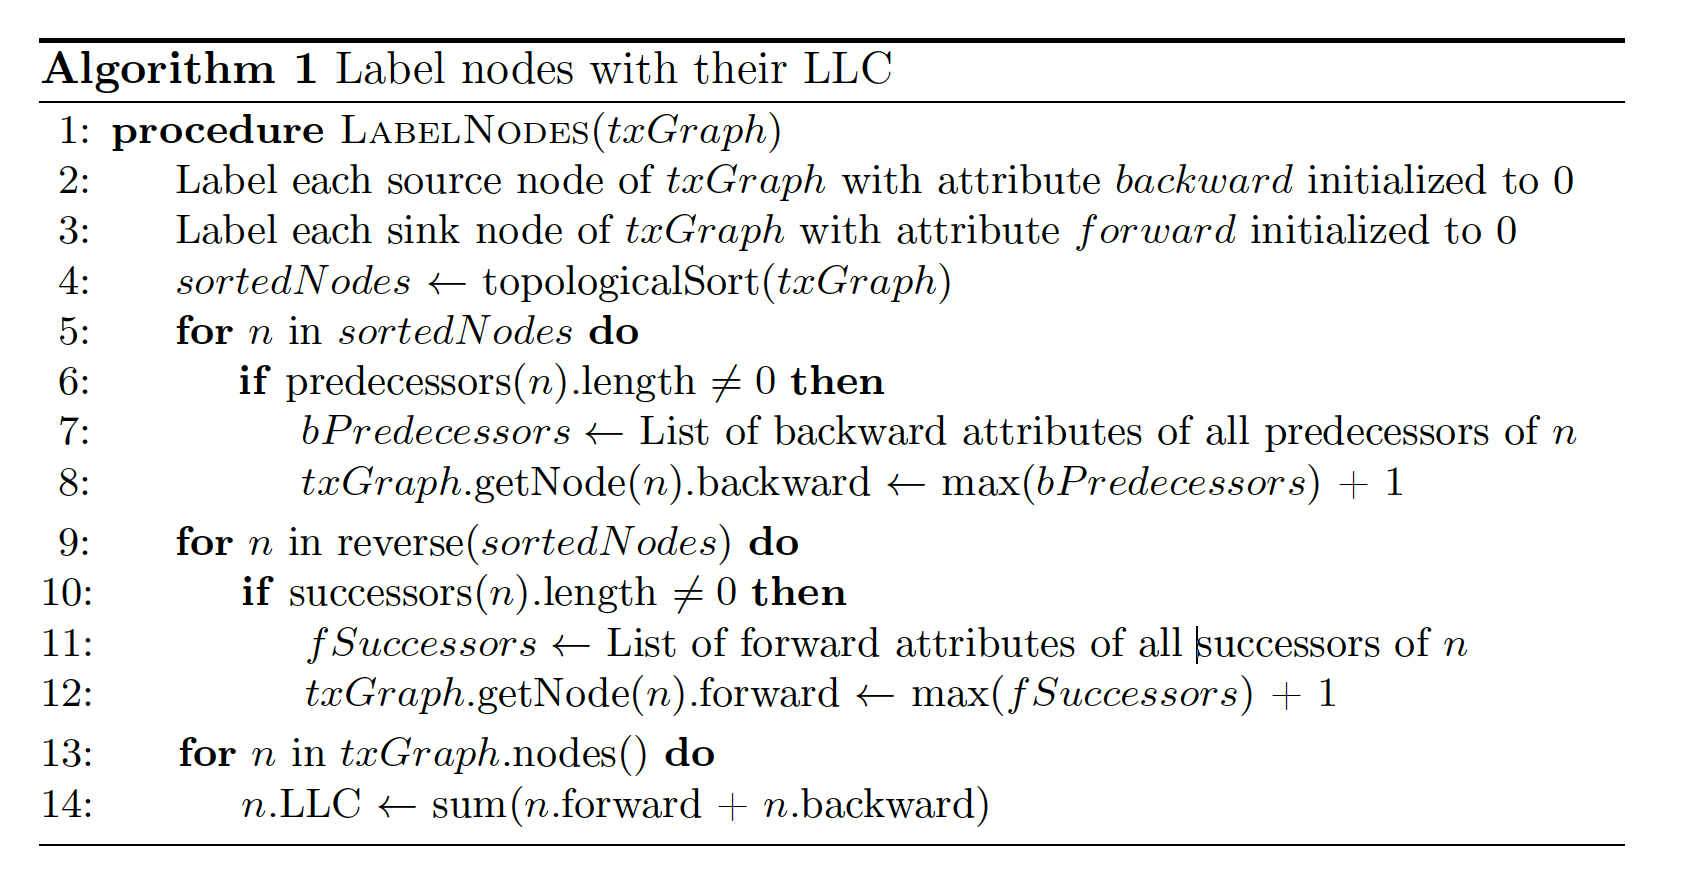
\includegraphics[width = \linewidth]{figure/llcalgo}
	\caption{\textit{Algoritmo assegnazione LLC} \cite{ddp-ltcbh-17} \label{fig:llcalgo}}
\end{figure}

